\documentclass[aspectratio=169]{beamer}

\usepackage[utf8]{inputenc}
\usepackage[brazil]{babel}
\usepackage{graphicx}
\usepackage{hyperref}
\usepackage{listings}

% Tema simples e limpo
\usetheme{Madrid}
\usecolortheme{default}
\setbeamertemplate{navigation symbols}{}

\graphicspath{{./imagens/}}

% -------------------------------------------------
% INFORMAÇÕES DO EP (OS ALUNOS DEVEM EDITAR)
% -------------------------------------------------

\title{MAC0209 --- Modelagem e Simulação}
\subtitle{EP 8 --- Cadeias de Markov}
\author[Grupo Plutão]{Grupo Plutão \\[4pt]
Guilherme França Carvalho \\
Ismália Alves Santos Ziemer \\
João Victor Bispo do Nascimento \\
Leonardo Heidi Almeida Murakami \\
Luis Renato Ferraz Natil Martins \\
Murilo Freitas Yonashiro Coelho \\
Vítor Gonçalves Serra \\
Vitor Wallace de Moraes Alves }
\institute[BCC IME-USP]{Bacharelado em Ciência da Computação \\ IME -- USP}
\date{\today}

% -------------------------------------------------

\begin{document}

% =================================================
% SLIDE 1
% =================================================
\begin{frame}
\titlepage
\end{frame}

\begin{frame}{Contexto e Objetivo do EP}

\textbf{Contexto do curso}

\begin{itemize}
    \item Algoritmos aleatórios para estimação de valores que não podem ser
        obtidos analiticamente.
    \item Método de Monte Carlo
\end{itemize}

\vspace{0.5cm}

\textbf{Objetivo do EP}

\begin{itemize}
    \item Apresentar uma aplicação de Cadeias de Markov
    \item Analisar como Cadeias de Markov podem gerar frases em língua natural
\end{itemize}

\end{frame}

% =================================================
% SLIDE 2
% =================================================
\begin{frame}{Trabalho Realizado}

\textbf{Conceitos e implementação}

\begin{itemize}
    \item Processo estocástico: Cadeia de Markov
    \item O próximo estado depende apenas do estado atual (memória de primeira
        ordem)
    \item Geração de frases em português através de uma Gramática predefinida.
\end{itemize}

\begin{figure}[b]
    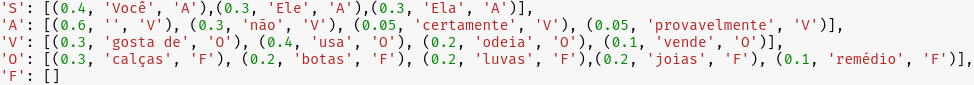
\includegraphics[width=0.8\textwidth]{img/grammar.png}
    \caption{Estados e Transições que definem a Gramática}
\end{figure}

\end{frame}

% =================================================
% SLIDE 3
% =================================================
\begin{frame}{Resultados e Conclusões}

\textbf{Resultados}

\begin{itemize}
    \item É possível gerar frases coesas em português através de uma Cadeia de Markov
    \item As transições e estados predefinidos formam as regras da Gramática
    \item A coerência das frases depende da rigorosidade das regras da Gramática
    \item Uma Gramática menos rigorosa pode gerar frases incoerentes
\end{itemize}

\begin{figure}[b]
    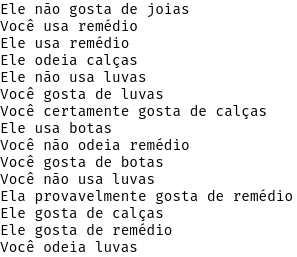
\includegraphics[height=0.25\textwidth]{img/resultado.png}
    \caption{Frases geradas por uma Cadeia de Markov como uma Gramática Estocástica}
\end{figure}

\end{frame}

\end{document}
